\documentclass[12pt]{article}
\usepackage[utf8]{inputenc}
\usepackage{geometry}
\usepackage{amsfonts}
\usepackage{hyperref}
\usepackage{enumitem}
\usepackage{graphicx}
\usepackage{tabularx}
\usepackage{amsmath}
\usepackage{xcolor}
\usepackage{array}
\usepackage{tikz}


\title{
    \textbf{CSE643: Artificial Intelligence} \\ \vspace*{-5pt}
    \textbf{\large{Assignment-1}}
}

\author{\href{mailto:divyajeet21529@iiitd.ac.in}{Divyajeet Singh (2021529)}}
\date{\today}

\geometry{a4paper, left=20mm, right=20mm, top=20mm, bottom=20mm}


\begin{document}
    \maketitle

    \section*{Theory}

    \subsection*{Problem-1}
    \textbf{(a)}
    The given text is composed of four sentences. Let us call them $S_{1}, S_{2}, S_{3}, S_{4}$ respectively.
    Let us define the following propositions
    \begin{enumerate}
        \item $A$: The universe simply exists as it is
        \item $B$: The universe ends in a heat death
        \item $C$: There was a big bang
        \item $D$: The universe is expanding
        \item $E$: The universe is accelerated
    \end{enumerate}
    Then, the given sentences are as follows
    \begin{align}
        \label{eq:s1}
        S_{1} &= A \vee B \equiv \lnot A \implies B \\
        \label{eq:s2}
        S_{2} &= \lnot C \implies A \equiv C \vee A \\
        \label{eq:s3}
        S_{3} &= D \Longleftrightarrow C \equiv (D \implies C) \wedge (C \implies D) \\
        \label{eq:s4}
        S_{4} &= (D \wedge E) \implies B
    \end{align}
    \vspace*{0pt} \\
    \textbf{(b)}
    The contrapositives of the sentences are
    \begin{align*}
        S_{1} &= \lnot B \implies A \\
        S_{2} &= \lnot A \implies C \\
        S_{3} &= (\lnot C \implies \lnot D) \wedge (\lnot D \implies \lnot C) \equiv \lnot C \Longleftrightarrow \lnot D \\
        S_{4} &= \lnot B \implies \lnot (D \wedge E) \equiv \lnot B \implies (\lnot D \vee \lnot E)
    \end{align*}
    \vspace*{0pt} \\
    \textbf{(c)}
    If $B$ is \textsc{False}, then at least one of $D$ or $E$ must be \textsc{False} by \eqref{eq:s4}. If $D$ is \textsc{False}, then $C$ must be \textsc{False}
    by \eqref{eq:s3}. Finally, by \eqref{eq:s2} and \eqref{eq:s1}, $A$ must be \textsc{True}. Hence, \textbf{we can infer that}
    either the universe is not expanding or the universe is not accelerated if the universe does not end in a heat death. Also,
    if the universe is not expanding, then there was no big bang and the universe simply exists as it is. \\
    If $A$ is \textsc{False}, then $B$ and $C$ must be \textsc{True} by \eqref{eq:s1} and \eqref{eq:s2} respectively. Then,
    by \eqref{eq:s3}, $D$ must be \textsc{True}. But since $B$ is \textsc{True}, the implication in \eqref{eq:s4} is vacuously
    \textsc{True}. So we cannot determine the truth value of $E$. This means that \textbf{we cannot infer} whether the universe
    is accelerated or not if the universe does not simply exist as it is. \\
    \vspace*{0pt} \\
    \textbf{(d)}
    The AND-OR graph of the statements is given in Figure \ref{fig:and-or}.
    \begin{figure}[htpb]
        \centering
        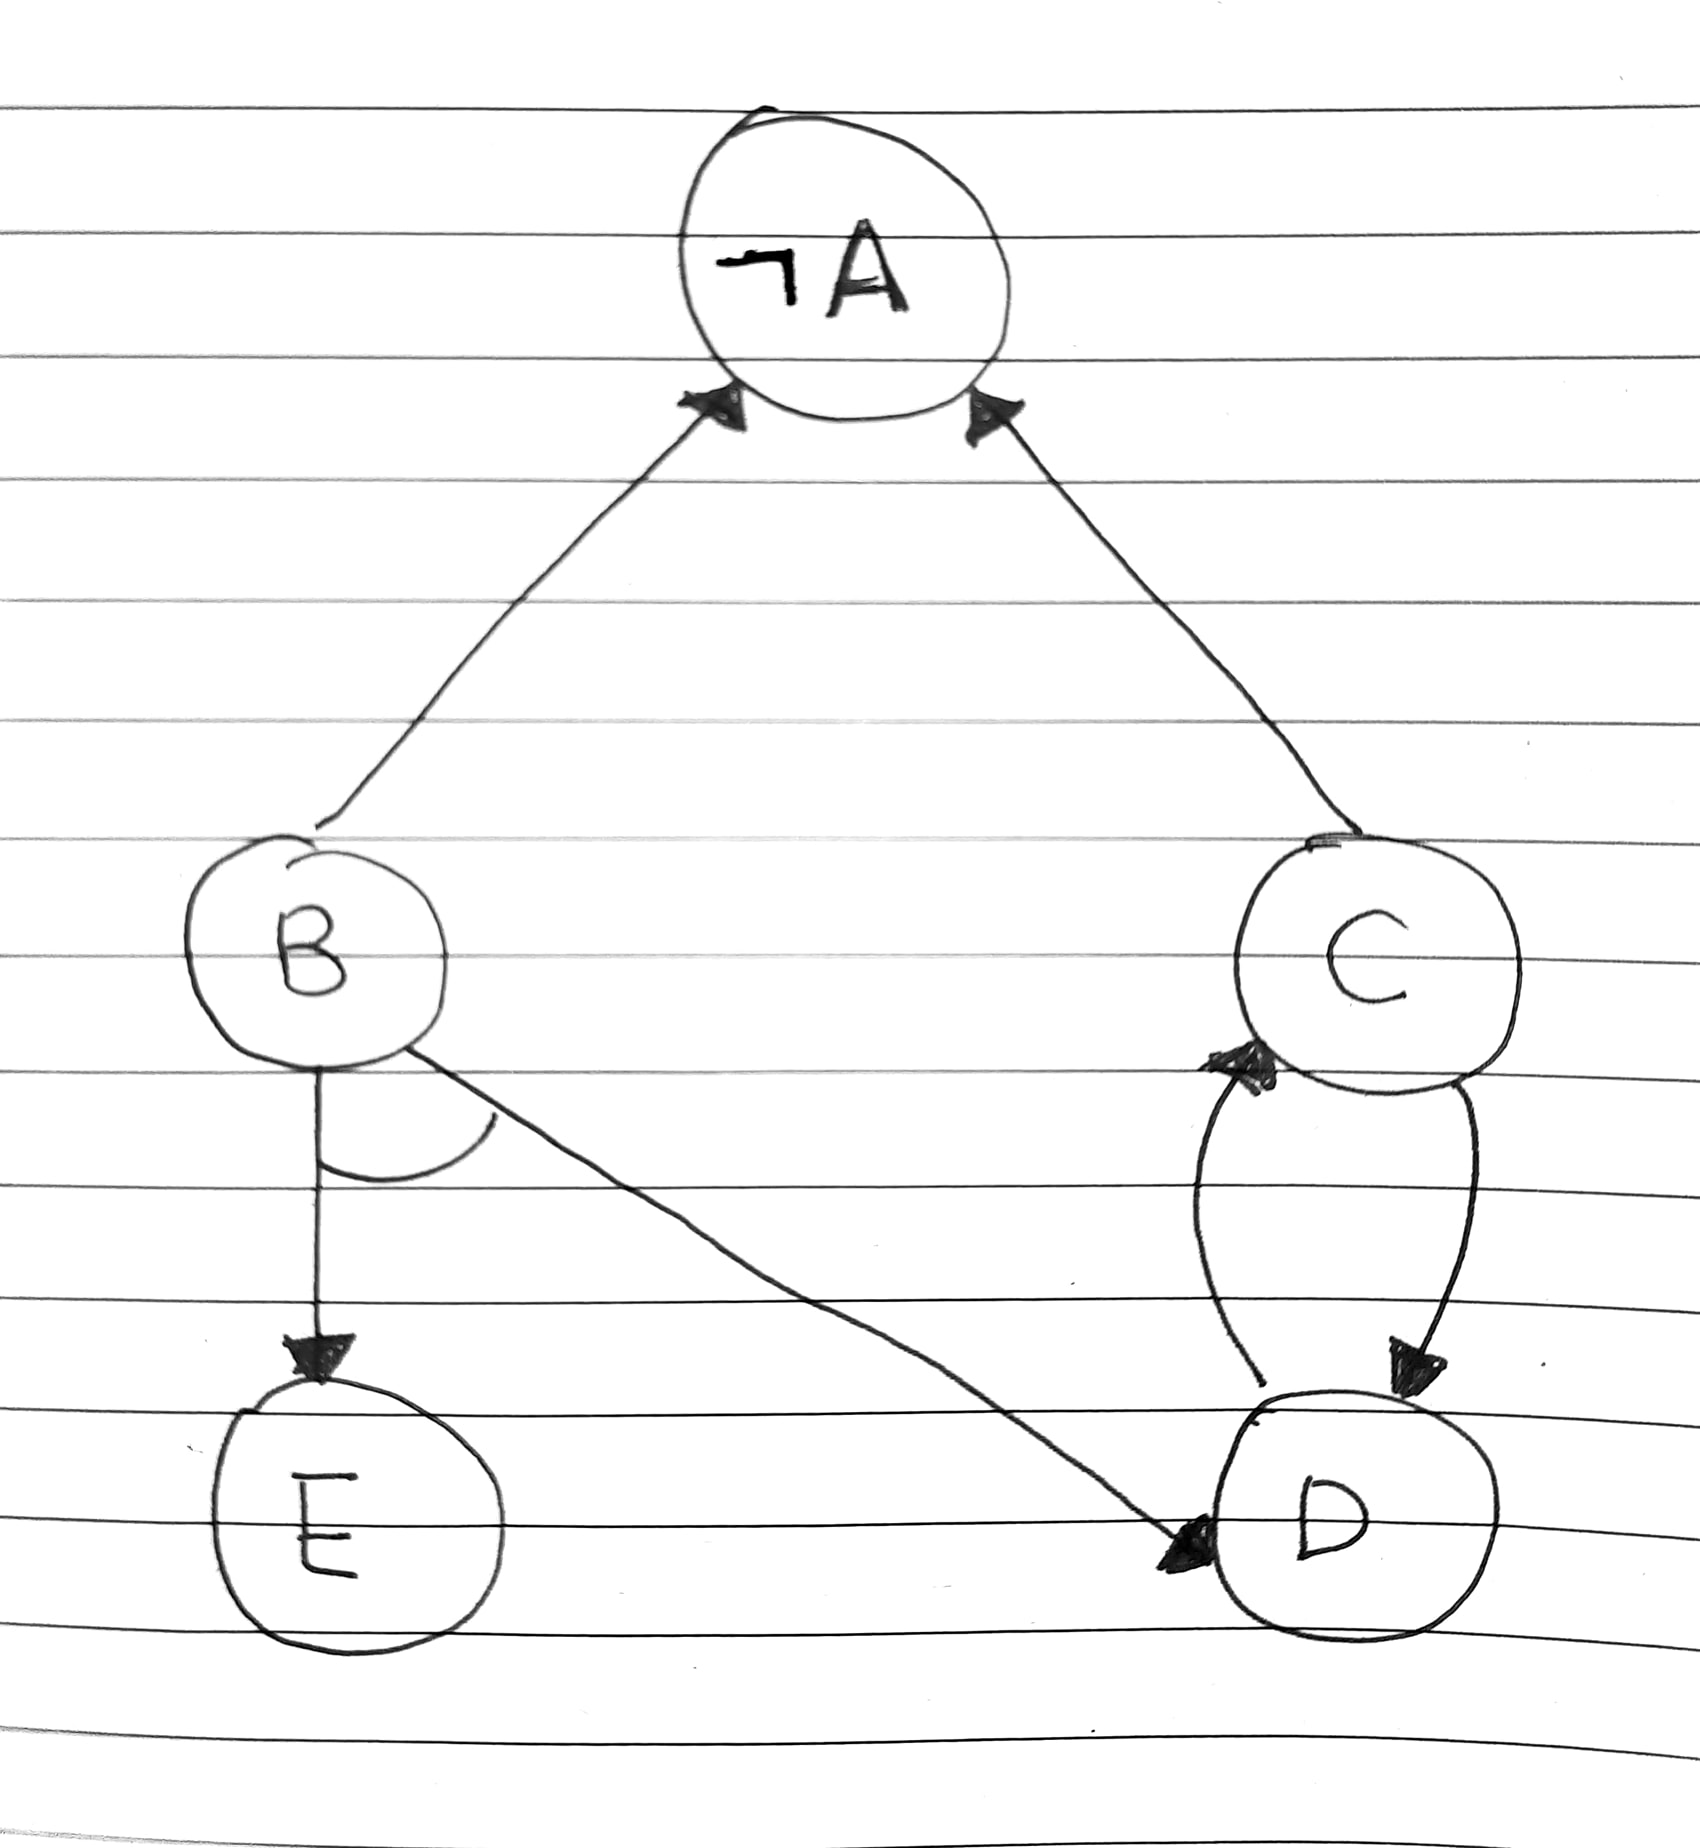
\includegraphics[width=0.35\textwidth]{Assets/and-or.jpg}
        \caption{And-OR Graph of the Statements}
        \label{fig:and-or}
    \end{figure}
    This graph is in accordance with the notation given on the
    \href{https://en.wikipedia.org/wiki/And%E2%80%93or_tree}{\underline{Wikipedia page - And-OR Tree}}.

    \subsection*{Problem-2}
    The required semantic network is given in Figure \ref{fig:semantic-net}.
    \begin{figure}[htbp]
        \centering
        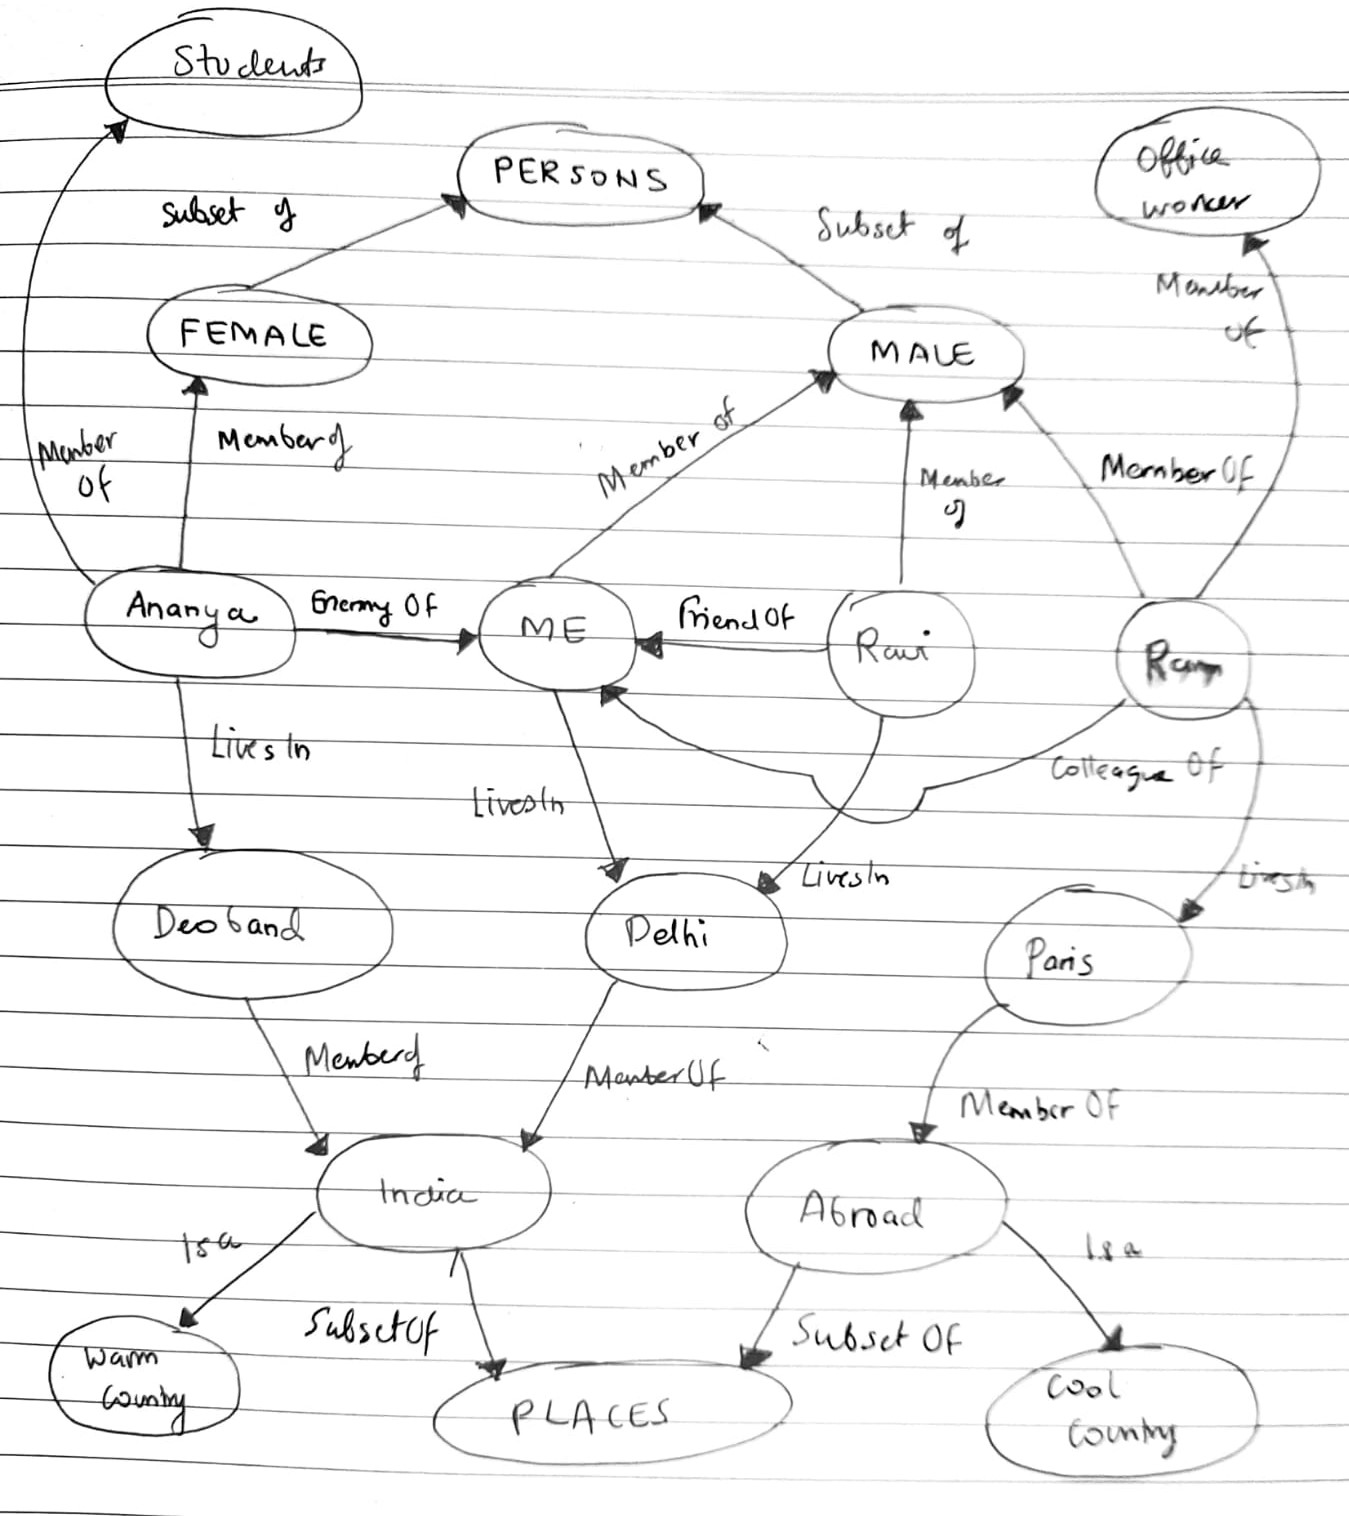
\includegraphics[width=0.574\textwidth]{Assets/semantic-net.jpg}
        \caption{Semantic Network of my relationships with 3 individuals}
        \label{fig:semantic-net}
    \end{figure}
    The centeral (labelled) node represents myself. The other three nodes with names represent three individuals
    with whom I share a relationship. The edges represent and are labelled as \textit{MemberOf}, \textit{SubsetOf},
    etc. to denote the relationship between the two nodes. \\[5pt]
    \textbf{Inheritance:} \\
    An example of Inheritance can be found in the part of the semantic diagram showing
    locations. The node \textit{India} has an attribute indicating it is a Warm Country. Similarly,
    the node \textit{Abroad} is labelled as Cool. So, by inheritance, the members of these
    classes inherit these properties - i.e. Deoband is a warm place and so is Delhi, while Paris
    is a cool place. \\[5pt]
    \textbf{Multiple Inheritance:} \\
    An example of Multiple Inheritance can be found in the part of the semantic diagram showing
    the persons. The node \textit{Ananya} belongs to the class \textit{Female} as well as \textit{Student}, so
    it can display properties of both. Similarly, the node \textit{Ram} is both \textit{Male} and an
    \textit{Office Worker}.

    \subsection*{Problem-3}
    Proof by resolution technique works by resolving complementary literals iteratively from a set
    of clauses until either the empty clause is obtained or no further resolution is possible.
    This is formally written as the inference rule
    $$\frac
    {l_{1} \vee \cdots \vee l_{k}, \quad m_{1} \vee \cdots \vee m_{n}}
    {l_{1} \vee \cdots \vee l_{i-1} \vee l_{i+1} \vee \cdots \vee l_{k} \vee m_{1} \vee \cdots
    \vee m_{j-1} \vee m_{j+1} \vee \cdots \vee m_{n}}$$
    where $l_{i}$ and $m_{j}$ form a pair of complementary literals. We now show that the method of
    inference by resolution is sound and complete.

    \subsubsection*{Proof for Soundness}
    The \textit{soundness} of proof by resolution can be shown easily. Let $l_{i}$ and $m_{j}$ be
    two complementary literals as above. Given the two clauses
    \begin{align}
        \label{eq:ls}
        l_{1} &\vee \cdots \vee l_{k} \\
        \label{eq:ms}
        m_{1} &\vee \cdots \vee m_{n}
    \end{align}
    Since $l_{i}$ and $m_{j}$ are complementary literals, $l_{i}$ is \textsc{True} when $m_{j}$ is \textsc{False} and
    vice versa. Let us consider the two cases.
    \begin{enumerate}
        \item
        $l_{i}$ is \textsc{False}. Then, $l_{1} \vee \cdots \vee l_{i-1} \vee l_{i+1} \vee \cdots \vee l_{k}$ must be
        \textsc{True} because \eqref{eq:ls} is given. This makes the inferred clause \textsc{True}.
        \item
        $l_{i}$ is \textsc{True}, i.e. $m_{j}$ is \textsc{False}. Then,
        $m_{1} \vee \cdots \vee m_{j-1} \vee m_{j+1} \vee \cdots \vee m_{n}$ must be \textsc{True} because \eqref{eq:ms}
        is given. This suggests that the inferred clause is \textsc{True}.
    \end{enumerate}

    \subsubsection*{Proof for Completeness}
    With the assumption that the knowledge base $\mathbb{K}$ is in CNF form, the \textit{completeness} of proof by
    resolution can also be shown easily. Let $\Sigma$ be the set of all clauses of the (say) $k$ symbols from $\mathbb{K}$.
    Then, let $\Omega(\Sigma)$ be the closure of $\Sigma$ under the resolution rule\footnote{
        $\Omega(\Sigma)$ is finite, since only a finite number of clauses can be generated from a finite $\Sigma$.
    }. The \textit{completeness} is proved using Ground Resolution Theorem, which states that if $\Omega(\Sigma)$ does not
    contain the empty clause, then $\Sigma$ is satisfiable. \\
    To prove this, we construct a model $\mathbf{P}_{1:k} = P_{1}, \hdots, P_{k}$ for $\Sigma$. For each symbol $P_{i}$,
    assign \textsc{False} if some clause in $\Omega(\Sigma)$ uses $\lnot P_{i}$ and all its other literals are \textsc{False}
    under the model $\mathbf{P}_{1:i-1}$. Otherwise, assign \textsc{True}. \\
    For the sake of contradiction, let us assume that at stage $j$, assigning symbol $P_{j}$ causes some clause $\theta$
    to become \textsc{False}. This means that all other literals in $\theta$ must be assigned \textsc{False} under the
    model $\mathbf{P}_{1:j-1}$. Therefore, $\theta$ must be one of the two forms
    \begin{align}
        \label{eq:pj}
        \textsc{False} &\vee \textsc{False} \vee \cdots \vee \textsc{False} \vee P_{j} \\
        \label{eq:pj-not}
        \textsc{False} &\vee \textsc{False} \vee \cdots \vee \textsc{False} \vee \lnot P_{j}
    \end{align}
    Clearly, both clauses must be in $\Omega(\Sigma)$, otherwise the procedure would assign an appropriate value to $P_{j}$.
    Since $\Omega(\Sigma)$ is closed under resolution, there must be some clause $\theta'$ in $\Omega(\Sigma)$ that is
    the resolvent of \eqref{eq:pj} and \eqref{eq:pj-not}. This resolvent will already have its literals $P_{1}, \hdots, P_{j-1}$
    assigned to \textsc{False}. This contradicts our assumption that the first falsified clause appears at stage $j$. So,
    the construction produces a model for $\Omega(\Sigma)$. Since $\Sigma \subseteq \Omega(\Sigma)$, $\mathbf{P}_{1:k}$ is
    also a model for $\Sigma$; and since it is a satisfying assignment, $\Sigma$ is satisfiable.

    \section*{Computational}
    The solution to the computational part of the assignment is given in the code in \texttt{main.py} in the submission.
    The code builds a recommender system for vacation destinations in great detail. The following attributes have been
    considered for decision making and wirting clauses in the code:
    \begin{enumerate}
        \item Weather of the destination
        \item The budget of the user
        \item The modes of connectivity to the destination
        \item The tourist activities available at the destination
        \item Rating of the destination
    \end{enumerate}
    The user can also add and view feedback for places - thereby explicitly modifying the
    knowledge base. The knowledge base is stored in the file \texttt{database.json} in the submission.
    This JSON file stores information about various destinations.

\end{document}